\documentclass[a4paper,10pt]{exam}
\usepackage{graphicx}
\usepackage[document]{ragged2e}
 \usepackage[margin=1in]{geometry}
\usepackage{circuitikz}
\pagestyle{empty}
\usepackage{tikz}
\usepackage{multirow}
\usepackage{float}
\usepackage{amsmath}
\usepackage{multicol}
\usepackage{array}
\usepackage{enumitem}
\usepackage{setspace}
\usepackage{amssymb}

\usepackage{cite}
\usepackage{graphicx}
\usepackage{amsmath,amssymb,amsfonts,amsthm}
\usepackage{algorithmic}
\usepackage{graphicx}
\usepackage{textcomp}
\usepackage{xcolor}
\usepackage{txfonts}
\usepackage{listings}
\usepackage{enumitem}
\usepackage{mathtools}
\usepackage{gensymb}
\usepackage{comment}
\usepackage[breaklinks=true]{hyperref}
\usepackage{tkz-euclide} 
\usepackage{listings}
\usepackage{gvv}                                        
%\def\inputGnumericTable{}                                 
\usetikzlibrary{arrows.meta, positioning}
\usepackage{xparse}
\usepackage{color}                                            
\usepackage{array}                                            
\usepackage{longtable}                                       
\usepackage{calc}                                             
\usepackage{multirow}
\usepackage{multicol}
\usepackage{hhline}                                           
\usepackage{ifthen}                                           
\usepackage{lscape}
\usepackage{tabularx}
\usepackage{array}
\usepackage{float}
\newtheorem{theorem}{Theorem}[section]
\newtheorem{problem}{Problem}
\newtheorem{proposition}{Proposition}[section]
\newtheorem{lemma}{Lemma}[section]
\newtheorem{corollary}[theorem]{Corollary}
\newtheorem{example}{Example}[section]
\newtheorem{definition}[problem]{Definition}
\newcommand{\BEQA}{\begin{eqnarray}}
\newcommand{\EEQA}{\end{eqnarray}}
\usepackage{float}
%\newcommand{\define}{\stackrel{\triangle}{=}}
\theoremstyle{remark}
\usepackage{circuitikz}
\usepackage{tikz}
\usepackage{ragged2e}
\begin{document}

\raggedright{2011}
\hfill
\raggedleft{Question Booklet Code : \textbf{A}}\\

\noindent\rule{\textwidth}{0.4pt}

\centering{\textbf{ EE :ELECTRICAL ENGINEERING}}\\
\vspace{0.5cm}
\raggedright{Duration:Three Hours} \hfill Maximum Marks: 100\\
\raggedright{\textbf{Read the following instructions carefully.}}
\vspace{0.1cm}

\begin{enumerate}[leftmargin=0.5cm,label=\arabic*.]
\item Do not open the seal of the Question Booklet until you are asked to do so by the invigilator.
\item Take out the Optical Response Sheet (\textbf{ORS}) from this Question Booklet \textbf{without breaking the seal}.
If you find that the Question Booklet Code printed at the right hand top corner of this page does not match with the Booklet Code on the \textbf{ORS}, exchange the booklet immediately with a new sealed Question Booklet.
\item Write your registration number, your name and name of the examination centre at the specified locations on the right half of the \textbf{ORS}. Also, using HB pencil, darken the appropriate bubble under each digit of your registration number and the letters corresponding to your test paper code (EE).
\item Write your name and registration number in the space provided at the bottom of this page.
\item This Booklet contains \textbf{24 pages} including blank pages for rough work. After opening the seal at the specified time, please check all pages and report discrepancy, if any.
\item There are a total of 65 questions carrying 100 marks. All these questions are of objective type. Questions must be answered on the left hand side of the \textbf{ORS} by darkening the appropriate bubble (marked A, B, C, D) using HB pencil against the question number. \textbf{For each question darken the bubble of the correct answer.} In case you wish to change an answer, erase the old answer completely. More than one answer bubbled against a question will be treated as an incorrect response.
\item Questions Q.1 -- Q.25 carry 1-mark each, and questions Q.26 -- Q.55 carry 2-marks each.
\item Questions Q.48 -- Q.51 (2 pairs) are common data questions and question pairs (Q.52, Q.53) and (Q.54, Q.55) are linked answer questions. The answer to the second question of the linked answer questions depends on the answer to the first question of the pair. If the first question in the linked pair is wrongly answered or is unattempted, then the answer to the second question in the pair will not be evaluated.
\item Questions Q.56 -- Q.65 belong to General Aptitude (GA). Questions Q.56 -- Q.60 carry 1-mark each, and questions Q.61 -- Q.65 carry 2-marks each. The GA questions begin on a fresh page starting from page \textbf{17}.
\item Unattempted questions will result in zero mark and wrong answers will result in \textbf{NEGATIVE} marks. For Q.1 -- Q.25 and Q.56 -- Q.60, $\frac{1}{3}$ mark will be deducted for each wrong answer. For Q.26 -- Q.51 and Q.61 -- Q.65, $\frac{2}{3}$ mark will be deducted for each wrong answer. The question pairs (Q.52, Q.53) and (Q.54, Q.55) are questions with linked answers. There will be negative marks only for wrong answer to the first question of the linked answer question pair, i.e. for Q.52 and Q.54, $\frac{2}{3}$ mark will be deducted for each wrong answer. There is no negative marking for Q.53 and Q.55.
\item Calculator is allowed whereas charts, graph sheets or tables are \textbf{NOT} allowed in the examination hall.
\item Rough work can be done on the question paper itself. Additionally, blank pages are provided at the end of the question paper for rough work.
\end{enumerate}
\begin{tabular}{|l|l|c|c|c|c|c|c|c|}
    \hline
    \multicolumn{1}{|c|}{\textbf{Name}} & \multicolumn{8}{l|}{} \\
    \hline
    \multicolumn{1}{|c|}{\textbf{Registration Number}} & \multicolumn{1}{c|}{EE} & & & & & & & \\
    \hline
\end{tabular}\\

\vspace{1cm}
\noindent\rule{\textwidth}{0.4pt}

\raggedright{EE-A}
\hfill
1/24

\newpage

\raggedright{2011}
\hfill
\raggedleft{EE}\\

\noindent\rule{\textwidth}{0.4pt}
\raggedright{\textbf{Q.1 - Q.25 carry one mark each.}}

\vspace{0.4cm}

\begin{enumerate}
    

\item \quad Roots of the algebraic equation $
x^3 + x^2 + x + 1 = 0
$ are\hfill{(GATE EE 2011)}

\begin{multicols}{4}
\begin{enumerate}
    \item $(+1, +j, -j)$
\item $(+1, -1, +1)$
\item $(0, 0, 0)$
\item $(-1, +j, -j)$
\end{enumerate}
\end{multicols}

\item \quad With $K$ as a constant, the possible solution for the first order differential equation
$
\frac{dy}{dx} = e^{-3x}
$
is\hfill{(GATE EE 2011)}

\begin{multicols}{4}
\begin{enumerate}
   \item $-\dfrac{1}{3}e^{-3x} + K$
\item $-\dfrac{1}{3}e^{3x} + K$
\item $-3e^{-3x} + K$
\item $-3e^{-x} + K$
\end{enumerate}
\end{multicols}

\item \quad The r.m.s value of the current $i(t)$ in the circuit shown below is\hfill{(GATE EE 2011)}

\begin{figure}[H]
    \centering
    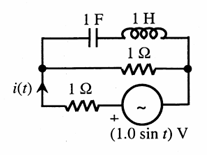
\includegraphics[width=0.2\columnwidth]{figs/Q 3.png}\caption{}     \label{fig:myfigure}
\end{figure}
\begin{multicols}{4}
\noindent (A) $\dfrac{1}{2}$A \\
\noindent (B)$\frac{1}{\sqrt{2}}$A\\
\noindent (C) $1$A \\
\noindent (D) $\sqrt{2}$A
\end{multicols}
\item \quad The Fourier series expansion $
f(t) = a_0 + \sum_{n=1}^{\infty} a_n \cos n\omega t + b_n \sin n\omega t
$
of the periodic signal shown below will contain the following nonzero terms \hfill{(GATE EE 2011)}
\begin{figure}[H]
    \centering
    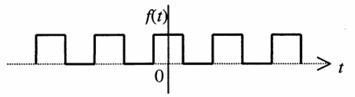
\includegraphics[width=0.3\columnwidth]{figs/Q 4.png}\caption{}     \label{fig:myfigure}
\end{figure}
\begin{multicols}{2}
(A) $a_0$ and $b_n$, $n=1,\,3,\,5,\ldots\infty$ \\

(C) $a_0,\, a_n$ and $b_n$, 
$n=1,\,2,\,3,\ldots\infty$ \\
(B) $a_0$ and $a_n$, $n=1,\,2,\,3,\ldots\infty$ \\

(D) $a_0$ and $a_n$, $n=1,\,3,\,5,\ldots\infty$
\end{multicols}

\item \quad A 4-point starter is used to start and control the speed of a\hfill{(GATE EE 2011)}

\begin{enumerate}
\item dc shunt motor with armature resistance control
\item dc shunt motor with field weakening control
\item dc series motor
\item dc compound motor
\end{enumerate}

\item \quad A three-phase, salient pole synchronous motor is connected to an infinite bus. It is operated at no load at normal excitation. The field excitation of the motor is first reduced to zero and then increased in the reverse direction gradually. Then the armature current\hfill{(GATE EE 2011)}

\begin{multicols}{2}
(A) increases continuously \\
(C) first decreases and then increases steeply \\[2ex]
(B) first increases and then decreases steeply \\

(D) remains constant
\end{multicols}
\vspace{1cm}
\noindent\rule{\textwidth}{0.4pt}
\raggedright{EE-A}
\hfill
2/24
\newpage
\raggedright{2011}
\hfill
\raggedleft{EE}\\

\noindent\rule{\textwidth}{0.4pt}

\item \quad A nuclear power station of $500$ MW capacity is located at $300$ km away from a load center. Select the most suitable power evacuation transmission configuration among the following options\hfill{(GATE EE 2011)}

\begin{figure}[H]
    \centering
    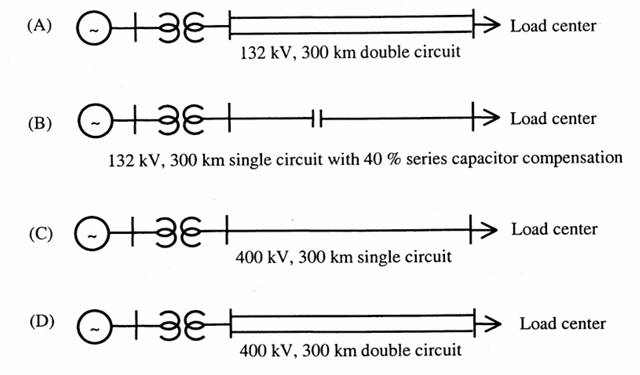
\includegraphics[width=0.7\columnwidth]{figs/Q 7.png}
\end{figure}

\item \quad The frequency response of a linear system $G(j\omega)$ is provided in the tabular form below

$
\begin{array}{|c|c|c|c|c|c|c|c|}
\hline
|G(j\omega)| & 1.3 & 1.2 & 1.0 & 0.8 & 0.5 & 0.3 \\
\hline
\angle G(j\omega) & -130^\circ & -140^\circ & -150^\circ & -160^\circ & -180^\circ & -200^\circ \\
\hline
\end{array}
$

The gain margin and phase margin of the system are \hfill{(GATE EE 2011)}

\begin{multicols}{4}
(A) 6 dB and $30^\circ$ \\
(B) 6 dB and $-30^\circ$ \\
(C) $-6$ dB and $30^\circ$ \\
(D) $-6$ dB and $-30^\circ$ 
\end{multicols}

\vspace{1em}

\item \quad The steady state error of a unity feedback linear system for a unit step input is $0.1$. The steady state error of the same system, for a pulse input $r(t)$ having a magnitude of $10$ and a duration of one second, as shown in the figure is\hfill{(GATE EE 2011)}


\begin{figure}[H]
        \centering
        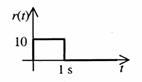
\includegraphics[width=0.2\columnwidth]{figs/Q 9.png}
        \caption{}
        \label{fig:placeholder}
    \end{figure}




\begin{multicols}{4}
(A) 0 \\
(B) 0.1 \\
(C) 1 \\
(D) 10 
\end{multicols}


\vspace{1em}

\item \quad Consider the following statements: \hfill{(GATE EE 2011)}\\
(i) The compensating coil of a low power factor wattmeter compensates the effect of the impedance of the current coil.\\
 (ii) The compensating coil of a low power factor wattmeter compensates the effect of the impedance of the voltage coil circuit.

\begin{multicols}{2}
\begin{enumerate}
     \item (i) is true but (ii) is false 
\item (i) is false but (ii) is true
\item both (i) and (ii) are true
\item both (i) and (ii) are false
\end{enumerate}
\end{multicols}

\vspace{1cm}
\noindent\rule{\textwidth}{0.4pt}
\raggedright{EE-A}
\hfill
3/24
\newpage
\raggedright{2011}
\hfill
\raggedleft{EE}\\

\noindent\rule{\textwidth}{0.4pt}

\item  A low-pass filter with a cut-off frequency of 30 Hz is cascaded with a high-pass filter with a cut-off frequency of 20 Hz. The resultant system of filters will function as\hfill{(GATE EE 2011)}
\begin{multicols}{2}
\begin{enumerate}
     \item an all-pass filter 
 \item an all-stop filter
 \item  a band stop (band-reject) filter 
 \item a band-pass filter
\end{enumerate}
\end{multicols}

\item For the circuit shown below,
\begin{figure}[H]
    \centering
    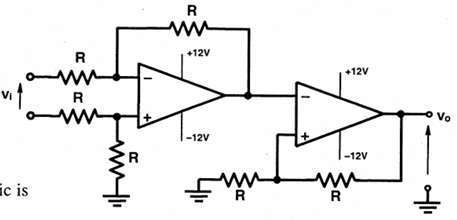
\includegraphics[width=0.7\columnwidth]{figs/Q 12.png}\caption{}     \label{fig:myfigure}
\end{figure}

the \textbf{CORRECT} transfer characteristic is\hfill{(GATE EE 2011)}

\begin{figure}[H]
    \centering
    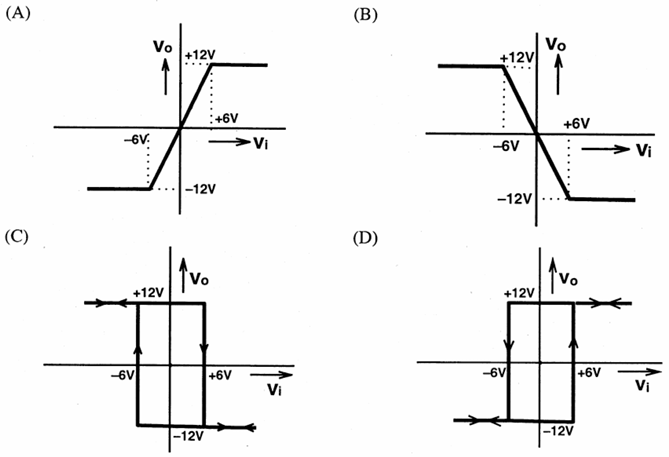
\includegraphics[width=0.9\columnwidth]{figs/Q 12 opt.png}
\end{figure}
\vspace{1cm}
\noindent\rule{\textwidth}{0.4pt}
\raggedright{EE-A}
\hfill
4/24
\newpage
\raggedright{2011}
\hfill
\raggedleft{EE}\\

\noindent\rule{\textwidth}{0.4pt}
\item \hspace{0.3cm} A three-phase current source inverter used for the speed control of an induction motor is to be realized using MOSFET switches as shown below. Switches $S_{1}$ to $S_{6}$ are identical switches.

\begin{figure}[H]
    \centering
    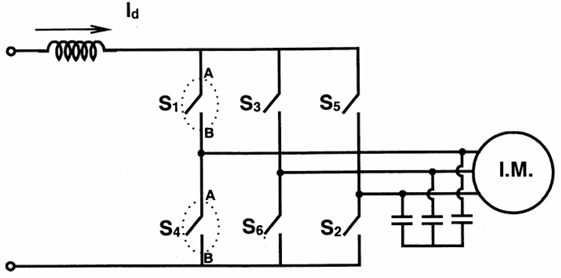
\includegraphics[width=0.6\columnwidth]{figs/Q 13.png}\caption{}     \label{fig:myfigure}
\end{figure}
\raggedright{The proper configuration for realizing switches  $S_{1}$ to $S_{6}$ is}\hfill{(GATE EE 2011)}
\begin{figure}[H]
    \centering
    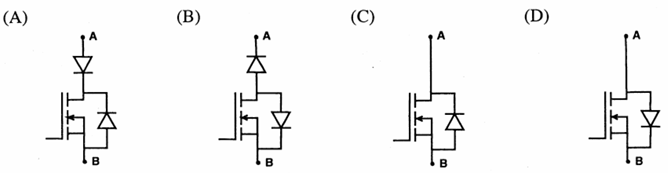
\includegraphics[width=0.75\columnwidth]{figs/Q 13 opt.png}
\end{figure}

\item A point Z has been plotted in the complex plane,as shown in the figure below.
\begin{figure}[H]
    \centering
    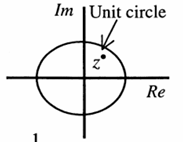
\includegraphics[width=0.2\columnwidth]{figs/Q 14.png}\caption{}     \label{fig:myfigure}
\end{figure}
The plot of the complex number y= $\frac{1}{z}$is\hfill{(GATE EE 2011)}
\begin{figure}[H]
    \centering
    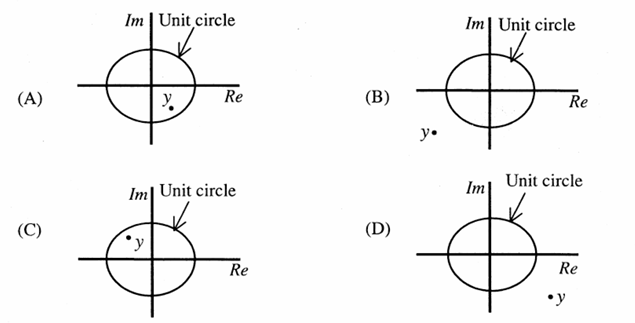
\includegraphics[width=0.6\columnwidth]{figs/Q 14 opt.png}
\end{figure}
\noindent\rule{\textwidth}{0.4pt}
\raggedright{EE-A}
\hfill
5/24
\newpage
\raggedright{2011}
\hfill
\raggedleft{EE}\\

\noindent\rule{\textwidth}{0.4pt}

\item The voltage applied to a circuit is $100\sqrt{2}\cos(100\pi t)$ volts and the circuit draws a current of $10\sqrt{2}\sin(100\pi t + \pi/4)$ amperes. Taking the voltage as the reference phasor, the phasor representation of the current in amperes is\hfill{(GATE EE 2011)}
\begin{multicols}{4}
\begin{enumerate}
    \item $10\sqrt{2} \angle -\pi/4$
    \item $10 \angle -\pi/4$
    \item $10 \angle +\pi/4$
    \item $10\sqrt{2} \angle +\pi/4$
\end{enumerate}
\end{multicols}

\item In the circuit given below, the value of R required for the transfer of maximum power to the load having a resistance of $3\Omega$ is\hfill{(GATE EE 2011)}
\begin{figure}[H]
    \centering
    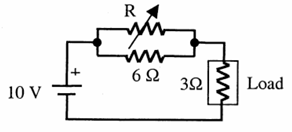
\includegraphics[width=0.5\columnwidth]{figs/Q 16.png}\caption{}     \label{fig:myfigure}
\end{figure}
\begin{multicols}{4}
\begin{enumerate}
    \item zero
    \item $3\Omega$ 
    \item  $6\Omega$
    \item infinity
\end{enumerate}
\end{multicols}

\item Given two continuous time signals $x(t) = e^{-t}$ and $y(t) = e^{-2t}$ which exist for $t > 0$, the convolution $z(t) = x(t) * y(t)$ is\hfill{(GATE EE 2011)}

\vspace{1em}

\begin{multicols}{4}
\begin{enumerate}
    \item $e^{-t} - e^{-2t}$
    \item $e^{-3t}$
    \item $e^{+t}$
    \item $e^{-t} + e^{-2t}$
\end{enumerate}
\end{multicols}

\item A single-phase air core transformer, fed from a rated sinusoidal supply, is operating at no load. The steady state magnetizing current drawn by the transformer from the supply will have the waveform\hfill{(GATE EE 2011)}


\begin{figure}[H]
    \centering
    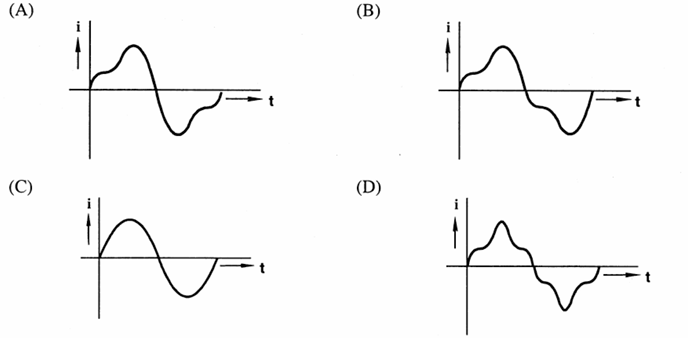
\includegraphics[width=0.8\columnwidth]{figs/Q 18.png}
\end{figure}

\item A negative sequence relay is commonly used to protect\hfill{(GATE EE 2011)}
\begin{multicols}{4}
\begin{enumerate}
    \item an alternator
    \item a transformer
    \item a transmission line
    \item a bus bar
\end{enumerate}
\end{multicols}

\vfill
\noindent\rule{\textwidth}{0.4pt}
\raggedright{EE-A}
\hfill
6/24
\newpage
\raggedright{2011}
\hfill
\raggedleft{EE}\\

\noindent\rule{\textwidth}{0.4pt}

\item For enhancing the power transmission in a long EHV transmission line, the most preferred method is to connect a\hfill{(GATE EE 2011)}
\begin{enumerate}
  \item series inductive compensator in the line
  \item shunt inductive compensator at the receiving end
  \item series capacitive compensator in the line
  \item shunt capacitive compensator at the sending end
\end{enumerate}

\item An open loop system represented by the transfer function $G(s)=\frac{(s-1)}{(s+2)(s+3)}$ is\hfill{(GATE EE 2011)}
\begin{multicols}{2}
\begin{enumerate}
  \item stable and of the minimum phase type
  \item stable and of the non-minimum phase type
  \item unstable and of the minimum phase type
  \item unstable and of the non-minimum phase type
\end{enumerate}
\end{multicols}

\item The bridge circuit shown in the figure below is used for the measurement of an unknown element $Z_{X}$. The bridge circuit is best suited when $Z_{X}$ is a\hfill{(GATE EE 2011)}
\begin{figure}[H]
    \centering
    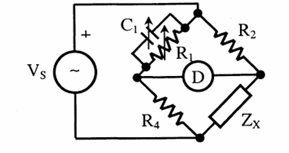
\includegraphics[width=0.4\columnwidth]{figs/Q 22.png}\caption{}     \label{fig:myfigure}
\end{figure}
\begin{multicols}{4}
\begin{enumerate}
  \item low resistance
  \item high resistance
  \item low Q inductor
  \item lossy capacitor
\end{enumerate}
\end{multicols}

\item A dual trace oscilloscope is set to operate in the ALTernate mode. The control input of the multiplexer used in the y-circuit is fed with a signal having a frequency equal to\hfill{(GATE EE 2011)}

\begin{enumerate}
  \item the highest frequency that the multiplexer can operate properly
  \item twice the frequency of the time base (sweep) oscillator
  \item the frequency of the time base (sweep) oscillator
  \item half the frequency of the time base (sweep) oscillator
\end{enumerate}


\item The output \textbf{Y} of the logic circuit given below is\hfill{(GATE EE 2011)}

\begin{figure}[H]
    \centering
    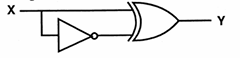
\includegraphics[width=0.4\columnwidth]{figs/Q 24.png}\caption{}     \label{fig:myfigure}
\end{figure}

\begin{multicols}{4}
\begin{enumerate}
  \item 1
  \item 0
  \item X
  \item $\overline{X}$
\end{enumerate}
\end{multicols}

\item \textit{Circuit turn-off time} of an SCR is defined as the time\hfill{(GATE EE 2011)}
\begin{enumerate}
  \item taken by the SCR to turn off
  \item required for the SCR current to become zero
  \item for which the SCR is reverse biased by the commutation circuit
  \item for which the SCR is reverse biased to reduce its current below the holding current
\end{enumerate}
\vfill
\noindent\rule{\textwidth}{0.4pt}
\raggedright{EE-A}
\hfill
7/24
\newpage
\raggedright{2011}
\hfill
\raggedleft{EE}\\

\noindent\rule{\textwidth}{0.4pt}


\raggedright{\textbf{Q. 26 to Q. 55 carry two marks each.}}

\vspace{0.5cm}

\item \quad Solution of the variables $x_1$ and $x_2$ for the following equations is to be obtained by employing the Newton-Raphson iterative method.\\

equation (i) \hspace{4cm}  $10 x_2 \sin x_1 - 0.8 = 0$ \\
equation (ii) \hspace{4cm} $10 x_2^2 - 10 x_2 \cos x_1 - 0.6 = 0$\\


Assuming the initial values $x_1=0.0$ and $x_2=1.0$, the Jacobian matrix is\hfill{(GATE EE 2011)}

\begin{multicols}{2}
\begin{enumerate}
\item $\myvec{ 10 & -0.8 \\ 0 & -0.6 }$
\item $\myvec{ 10 & 0 \\ 0 & 10 }$
\item $\myvec{ 0 & -0.8 \\ 10 & -0.6 }$
\item $\myvec{ 10 & 0 \\ 10 & -10 }$
\end{enumerate}
\end{multicols}

\item \quad The function $f(x)=2x-x^2+3$ has\hfill{(GATE EE 2011)}

\begin{multicols}{2}
\begin{enumerate}
\item a maxima at $x=1$ and a minima at $x=5$
\item a maxima at $x=1$ and a minima at $x=-5$
\item only a maxima at $x=1$
\item only a minima at $x=1$
\end{enumerate}
\end{multicols}

\item \quad A lossy capacitor $C_X$, rated for operation at 5 kV, 50 Hz is represented by an equivalent circuit with an ideal capacitor $C_P$ in parallel with a resistor $R_P$. The value of $C_P$ is found to be 0.102 $\mu$F and the value of $R_P=1.25$ M$\Omega$. Then the power loss and $\tan \delta$ of the lossy capacitor operating at the rated voltage, respectively, are\hfill{(GATE EE 2011)}

\begin{multicols}{2}
\begin{enumerate}
\item 10 W and 0.0002
\item 10 W and 0.0025
\item 20 W and 0.025
\item 20 W and 0.04
\end{enumerate}
\end{multicols}

\item \quad Let the Laplace transform of a function $f(t)$ which exists for $t>0$ be $F_1(s)$ and the Laplace transform of its delayed version $f(t - \tau)$ be $F_2(s)$. Let $F^*_1(s)$ be the complex conjugate of $F_1(s)$ with the Laplace variable set as $s = \sigma + j \omega$. If \\  \hspace*{2em} $G(s) = \dfrac{F_2(s) F^*_1(s)}{|F_1(s)|^2}$, then the inverse Laplace transform of $G(s)$ is\hfill{(GATE EE 2011)}

\begin{multicols}{2}
\begin{enumerate}
\item an ideal impulse $\delta(t)$
\item an ideal delayed impulse $\delta(t-\tau)$
\item an ideal step function $u(t)$
\item an ideal delayed step function $u(t-\tau)$
\end{enumerate}
\end{multicols}

\item \quad A zero mean random signal is uniformly distributed between limits $-a$ and $+a$ and its mean square value is equal to its variance. Then the r.m.s value of the signal is\hfill{(GATE EE 2011)}

\begin{multicols}{2}
\begin{enumerate}
\item $\dfrac{a}{\sqrt{3}}$
\item $\dfrac{a}{\sqrt{2}}$
\item $a\sqrt{2}$
\item $a\sqrt{3}$
\end{enumerate}
\end{multicols}

\item \quad A 220 V, DC shunt motor is operating at a speed of 1440 rpm. The armature resistance is 1.0 $\Omega$ and armature current is 10 A. If the excitation of the machine is reduced by 10\%, the extra resistance to be put in the armature circuit to maintain the same speed and torque will be\hfill{(GATE EE 2011)}

\begin{multicols}{2}
\begin{enumerate}
\item 1.79 $\Omega$
\item 2.1 $\Omega$
\item 3.1 $\Omega$
\item 18.9 $\Omega$
\end{enumerate}
\end{multicols}

\vfill
\noindent\rule{\textwidth}{0.4pt}
\raggedright{EE-A}
\hfill
8/24
\newpage
\raggedright{2011}
\hfill
\raggedleft{EE}\\

\noindent\rule{\textwidth}{0.4pt}

\item A load center of 120 MW derives power from two power stations connected by 220 kV transmission lines of 25 km and 75 km as shown in the figure below. The three generators G1, G2 and G3 are of 100 MW capacity each and have identical fuel cost characteristics. The \textit{minimum loss generation schedule} for supplying the 120 MW load is\hfill{(GATE EE 2011)}

\begin{figure}[H]
    \centering
    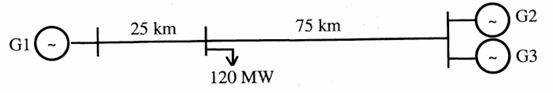
\includegraphics[width=1\columnwidth]{figs/Q 32.png}\caption{}     \label{fig:myfigure}
\end{figure}

\begin{multicols}{2}
\begin{enumerate}
  \item P1 = 80 MW + losses \\
        P2 = 20 MW \\
        P3 = 20 MW
  \item P1 = 60 MW \\
        P2 = 30 MW + losses \\
        P3 = 30 MW
  \item P1 = 40 MW \\
        P2 = 40 MW \\
        P3 = 40 MW + losses
  \item P1 = 30 MW + losses \\
        P2 = 45 MW \\
        P3 = 45 MW
\end{enumerate}
\end{multicols}

\item The open loop transfer function $G(s)$ of a unity feedback control system is given as,
$
G(s) = \frac{k \left(s+\frac{2}{3}\right)}{s^{2}(s+2)}.
$

From the root locus, it can be inferred that when $k$ tends to positive infinity,\hfill{(GATE EE 2011)}


\begin{enumerate}
  \item three roots with nearly equal real parts exist on the left half of the $s$-plane
  \item one real root is found on the right half of the $s$-plane
  \item the root loci cross the $j\omega$ axis for a finite value of $k$; $k \neq 0$
  \item three real roots are found on the right half of the $s$-plane
\end{enumerate}
\item \quad A portion of the main program to call a subroutine SUB in an 8085 environment is given below.\\
\centering{
\hspace{3cm}:\\
\hspace{3cm}:\\
\hspace{2.7cm} LXI \hspace{0.3cm}D, DISP\\
\hspace{1cm}LP:\hspace{1.2cm} CALL  SUB\\
\hspace{3cm}:\\
\hspace{3cm}:\\}
It is desired that control be returned to LP + DISP + 3 when the RET instruction is executed in the subroutine. The set of instructions that precede the RET instruction in the subroutine are\hfill{(GATE EE 2011)}

\begin{multicols}{2}
\begin{enumerate}
  \item POP    D \\
        DAD    H \\
        PUSH   D
        
  \item POP    H \\
        DAD    D \\
        INX    H \\
        INX    H \\
        INX    H \\
        PUSH   H
        
  \item POP    H \\
        DAD    D \\
        PUSH   H
        
  \item XTHL \\
        INX    D \\
        INX    D \\
        INX    D \\
        XTHL
\end{enumerate}
\end{multicols}




\vfill
\noindent\rule{\textwidth}{0.4pt}
\raggedright{EE-A}
\hfill
9/24
\newpage
\raggedright{2011}
\hfill
\raggedleft{EE}\\

\noindent\rule{\textwidth}{0.4pt}

\item  The transistor used in the circuit shown below has a $\beta$ of 30 and $I_{CBO}$ is negligible.\hfill{(GATE EE 2011)}
\begin{figure}[H]
    \centering
    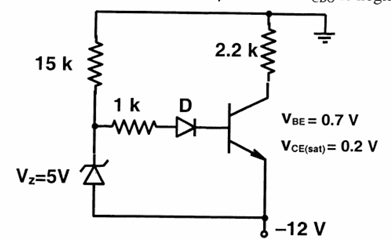
\includegraphics[width=0.75\columnwidth]{figs/Q 35.png}\caption{}     \label{fig:myfigure}
\end{figure}
\raggedright{If the forward voltage drop of diode is 0.7 V, then the current through collector will be}
\begin{multicols}{4}
\begin{enumerate}
  \item 168 mA
  \item 108 mA
  \item 20.54 mA
  \item 5.36 mA
\end{enumerate}
\end{multicols}
\item A voltage commutated chopper circuit, operated at 500 Hz, is shown below.\hfill{(GATE EE 2011)}

\begin{figure}[H]
    \centering
    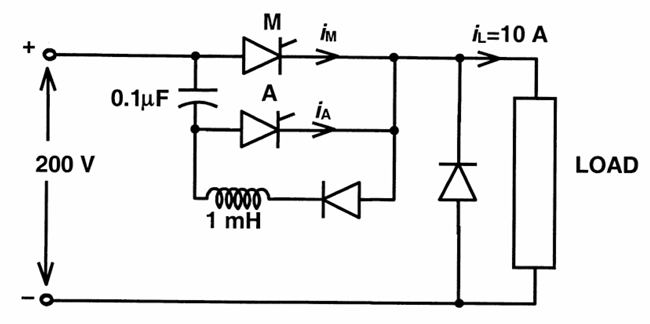
\includegraphics[width=0.8\columnwidth]{figs/Q 36.png}\caption{}     \label{fig:myfigure}
\end{figure}
If the maximum value of load current is 10A, then the maximum current through the main (M) and auxiliary (A) thyristors will be

\begin{multicols}{2}
\begin{enumerate}
\item $i_{M max}$ =12 A and  $i_{A max}$ =10 A
\item $i_{M max}$ =12 A and  $i_{A max}$ =2 A
\item $i_{M max}$ =10 A and  $i_{A max}$ =12 A
\item $i_{M max}$ =10 A and  $i_{A max}$ =8 A
\end{enumerate}
\end{multicols}

\vfill
\noindent\rule{\textwidth}{0.4pt}
\raggedright{EE-A}
\hfill
10/24
\newpage
\raggedright{2011}
\hfill
\raggedleft{EE}\\
\noindent\rule{\textwidth}{0.4pt}

\item The matrix [A] =$\myvec{ 2 & 1 \\ 4 & -1 } $is decomposed into a product of a lower triangular matrix [L] and an upper triangular matrix [U]. The properly decomposed [L] and [U] matrices respectively are\hfill{(GATE EE 2011)}

\begin{multicols}{2}
\begin{enumerate}
\item $\myvec{ 1 & 0 \\ 4 & -1 }$ and $\myvec{ 1 & 1 \\ 0 & -2 }$
\item $\myvec{ 2 & 0 \\ 4 & -1 }$ and $\myvec{ 1 & 1 \\ 0 & 1 }$
\item$\myvec{ 1 & 0 \\ 4 & 1 }$ and $\myvec{ 2 & 1 \\ 0 & -1 }$
\item $\myvec{ 2 & 0 \\ 4 & -3 }$ and $\myvec{ 1 & 0.5 \\ 0 & 1 }$
\end{enumerate}
\end{multicols}
\item\quad The two vectors [1,1,1] and [1,a,$a^2$], where a = $\left(
    -\frac{1}{2} + j \frac{\sqrt{3}}{2}
\right)$
, are \hfill{(GATE EE 2011)}

\begin{multicols}{4}
\begin{enumerate}
  \item orthonormal
  \item orthogonal
  \item parallel
  \item collinear
\end{enumerate}
\end{multicols}

\item A three-phase 440V, 6 pole, 50Hz, squirrel cage induction motor is running at a slip of 5\%. The speed of stator magnetic field with respect to rotor magnetic field and speed of rotor with respect to stator magnetic field are\hfill{(GATE EE 2011)}

\begin{multicols}{2}
\begin{enumerate}
\item zero, $-5$ rpm \item zero, $955$ rpm
\item $1000$ rpm, $-5$ rpm 
\item $1000$ rpm, $955$ rpm
\end{enumerate}
\end{multicols}

\item A capacitor is made with a polymeric dielectric having an $\varepsilon_r$ of $2.26$ and a dielectric breakdown strength of $50$ kV/cm. The permittivity of free space is $8.85$ pF/m. If the rectangular plates of the capacitor have a width of $20$cm and a length of $40$cm, then the maximum electric charge in the capacitor is\hfill{(GATE EE 2011)}
\begin{multicols}{4}
\begin{enumerate}
\item 2 $\mu$C
\item 4 $\mu$C
\item 8 $\mu$C
\item 10 $\mu$C
\end{enumerate}
\end{multicols}


\item \quad The response $h(t)$ of a linear time invariant system to an impulse $\delta(t)$, under initially relaxed condition is $h(t)=e^{-t} + e^{-2t}$. The response of this system for a unit step input $u(t)$ is\hfill{(GATE EE 2011)}

\begin{multicols}{2}
\begin{enumerate}
\item $u(t)+e^{-t}+e^{-2t}$
\item $\left(e^{-t}+e^{-2t}\right)u(t)$
\item $\left(1.5-e^{-t}-0.5e^{-2t}\right)u(t)$
\item  $e^{-t}\delta(t)+e^{-2t}u(t)$

\end{enumerate}
\end{multicols}



\item \quad The direct axis and quadrature axis reactances of a salient pole alternator are $1.2$p.u and $1.0$p.u respectively. The armature resistance is negligible. If this alternator is delivering rated kVA at upf and at rated voltage then its power angle is\hfill{(GATE EE 2011)}

\begin{multicols}{4}
\begin{enumerate}
\item $30^\circ$
\item $45^\circ$
\item $60^\circ$
\item $90^\circ$
\end{enumerate}
\end{multicols}
\vfill
\noindent\rule{\textwidth}{0.4pt}
\raggedright{EE-A}
\hfill
11/24
\newpage
\raggedright{2011}
\hfill
\raggedleft{EE}\\

\noindent\rule{\textwidth}{0.4pt}

\item \quad A $4\frac{1}{2}$ digit DMM has the error specification as: $0.2~\%$ of reading $+\,10$ counts. If a dc voltage of $100$ V is read on its $200$ V full scale, the maximum error that can be expected in the reading is\hfill{(GATE EE 2011)}
\begin{multicols}{4}
\begin{enumerate}

\item $\pm\,0.1~\%$
\item $\pm\,0.2~\%$
\item $\pm\,0.3~\%$
\item $\pm\,0.4~\%$

\end{enumerate}
\end{multicols}

\item \quad A three-bus network is shown in the figure below indicating the p.u. impedances of each element.
\begin{figure}[H]
    \centering
    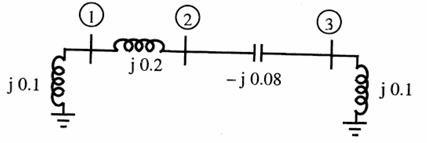
\includegraphics[width=0.7\columnwidth]{figs/Q 44.png}\caption{}     \label{fig:myfigure}
\end{figure}


The Bus admittance matrix, Y-bus, of the network is \hfill{(GATE EE 2011)}
\begin{multicols}{2}
\begin{enumerate}
\item \quad $j
\myvec{
0.3 & -0.2 & 0 \\
-0.2 & 0.12 & 0.08 \\
0 & 0.08 & 0.02
}$
\vspace{1.5em}
\item \quad $j
\myvec{
-15 & 5 & 0 \\
5 & 7.5 & -12.5 \\
0 & -12.5 & 2.5
}$

\vspace{1.5em}

\item \quad $j
\myvec{
0.1 & 0.2 & 0 \\
0.2 & 0.12 & -0.08 \\
0 & -0.08 & 0.10
}$

\vspace{1.5em}

\item \quad $j
\myvec{
-10 & 5 & 0 \\
5 & 7.5 & 12.5 \\
0 & 12.5 & -10
}$

\end{enumerate}
\end{multicols}

\item \quad A two-loop position position control system is shown below.\hfill{(GATE EE 2011)}

\begin{figure}[H]
    \centering
    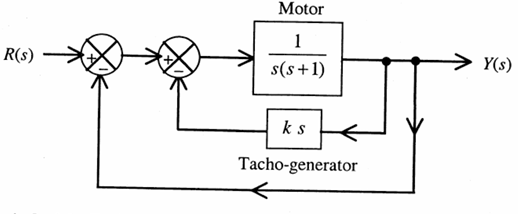
\includegraphics[width=0.75\columnwidth]{figs/Q 45.png}\caption{}     \label{fig:myfigure}
\end{figure}
\raggedright{The gain \textit{k} of the Tacho-generator influences mainly the}

\begin{enumerate}
\item peak overshoot
\item natural frequency of oscillation
\item phase shift of the closed loop transfer function at very low frequencies $(\omega \rightarrow 0)$
\item phase shift of the closed loop transfer function at very high frequencies $(\omega \rightarrow \infty)$
\end{enumerate}
\vfill
\noindent\rule{\textwidth}{0.4pt}
\raggedright{EE-A}
\hfill
12/24
\newpage
\raggedright{2011}
\hfill
\raggedleft{EE}\\

\noindent\rule{\textwidth}{0.4pt}

\item \quad A two-bit counter is shown below.\hfill{(GATE EE 2011)}
\begin{figure}[H]
    \centering
    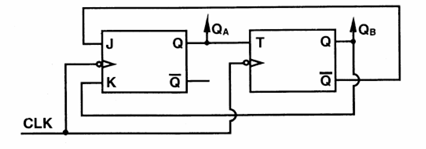
\includegraphics[width=0.75\columnwidth]{figs/Q 46.png}\caption{}     \label{fig:myfigure}
\end{figure}
If the state $Q_{A}Q_{B}$ of the counter at the clock time $t_{n}$ is "10" then the state $Q_{A}Q_{B}$ of the counter at $t_{n}$+3(after three clock cycles) will be 

\begin{multicols}{4}
\begin{enumerate}
\item $00$
\item $01$
\item $10$
\item $11$
\end{enumerate}
\end{multicols}
\item \quad A clipper circuit is shown below.\hfill{(GATE EE 2011)}
\begin{figure}[H]
    \centering
    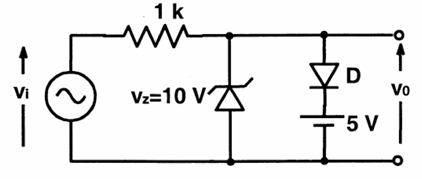
\includegraphics[width=0.4\columnwidth]{figs/Q 47.png}\caption{}     \label{fig:myfigure}
\end{figure}
Assuming forward voltage drops of the diodes to be 0.7V, the input-output transfer characteristics of the circuit is
\begin{figure}[H]
    \centering
    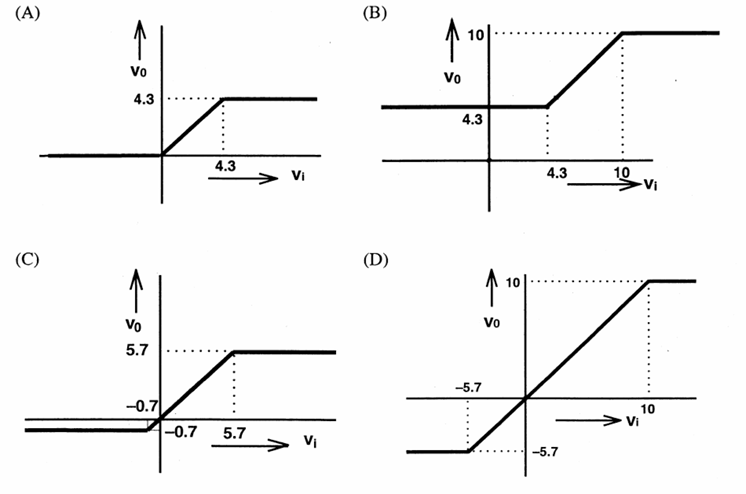
\includegraphics[width=0.7\columnwidth]{figs/Q 47 opt.png}
\end{figure}

\vfill
\noindent\rule{\textwidth}{0.4pt}
\raggedright{EE-A}
\hfill
13/24
\newpage
\raggedright{2011}
\hfill
\raggedleft{EE}\\

\noindent\rule{\textwidth}{0.4pt}
\raggedright{\textbf{Common Data Questions}}\\
\vspace{0.5cm}
\textbf{Common Data for  Questions 48 and 49:}\\
\vspace{0.1cm}
The input voltage given to a converter is \\
\hspace{3cm} $v_{i}= 100\sqrt{2}sin(100\pi t)  V$\\
\vspace{0.1cm}
The current drawn by the converter is \\
\hspace{3cm} $i_{i}= (10\sqrt{2}sin(100\pi t- \pi/3)+5\sqrt{2}sin(300\pi t+ \pi/4)+2\sqrt{2}sin(500\pi t- \pi/6))A $
\vspace{0.1cm}
\item \quad The input power factor of the converter is\hfill{(GATE EE 2011)}
\begin{multicols}{4}
\begin{enumerate}
\item $0.31$
\item $0.44$
\item $0.5$
\item $0.71$
\end{enumerate}
\end{multicols}
\item \quad The active power drawn by the converter is\hfill{(GATE EE 2011)}
\begin{multicols}{4}
\begin{enumerate}
\item $181 W$
\item $500 W$
\item $707 W$
\item $887 W$
\end{enumerate}
\end{multicols}
\textbf{Common Data for  Questions 50 and 51:}\\
An RLC circuit with relevant data is given below.
\begin{figure}[H]
    \centering
    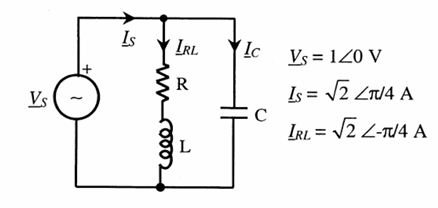
\includegraphics[width=0.8\columnwidth]{figs/Q 50,51.png}\caption{}     \label{fig:myfigure}
\end{figure}
\item \quad The power dissipated in the resistor R is \hfill{(GATE EE 2011)}
\begin{multicols}{4}
\begin{enumerate}
\item $0.5 W$
\item $1 W$
\item $\sqrt{2} W$
\item $2 W$
\end{enumerate}
\end{multicols}


\item \quad The current $I_{C}$ in the figure above is\hfill{(GATE EE 2011)}
\begin{multicols}{4}
\begin{enumerate}
\item $-j2A$
\item $-j \frac{1}{\sqrt{2}}A$
\item $+j \frac{1}{\sqrt{2}}A$
\item $+j2A$
\end{enumerate}
\end{multicols}

\vfill
\noindent\rule{\textwidth}{0.4pt}
\raggedright{EE-A}
\hfill
14/24
\newpage
\raggedright{2011}
\hfill
\raggedleft{EE}\\

\noindent\rule{\textwidth}{0.4pt}
\raggedright{\textbf{Linked Answer Questions}}\\
\vspace{0.4cm}
\textbf{Statement for Linked Answer Questions 52 and 53:}\\
\vspace{0.1cm}
Two generator units G1 and G2 are connected by 15 kV line with a bus at the mid-point as shown below.
\begin{figure}[H]
    \centering
    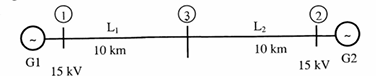
\includegraphics[width=0.7\columnwidth]{figs/Q 52,53.png}\caption{}     \label{fig:myfigure}
\end{figure}
G1 = 250 MVA, 15 kV, positive sequence reactance X = 25\%
 on its own base\\
G2 = 100 MVA, 15 kV, positive sequence reactance X = 10\%
 on its own base\\
$L_{1}$ and $L_{2}$ = 10 km, positive sequence reactance X = 0.225 $\Omega$/km\\
\item \quad For the above system, the positive sequence diagram with the p.u values on the 100 MVA common base is\hfill{(GATE EE 2011)}
\begin{figure}[H]
    \centering
    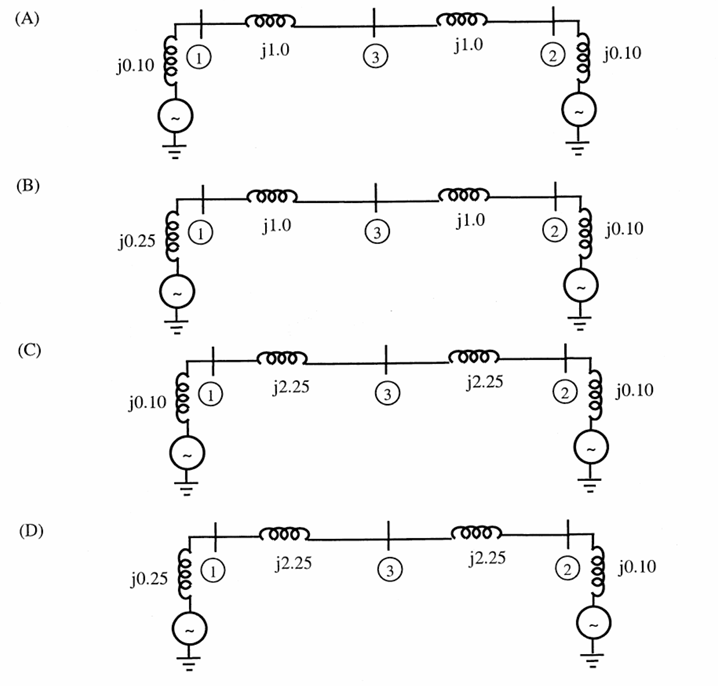
\includegraphics[width=0.8\columnwidth]{figs/Q 52 opt.png}
\end{figure}
\item \quad In the above system, the three-phase fault MVA at the bus 3 is \hfill{(GATE EE 2011)}
\begin{multicols}{4}
\begin{enumerate}
\item $82.55 MVA$
\item $85.11 MVA$
\item $170.91 MVA$
\item $181.82 MVA$
\end{enumerate}
\end{multicols}
\vfill
\noindent\rule{\textwidth}{0.4pt}
\raggedright{EE-A}
\hfill
15/24
\newpage
\raggedright{2011}
\hfill
\raggedleft{EE}\\

\noindent\rule{\textwidth}{0.4pt}

\raggedright{\textbf{Statement for Linked Answer Questions 52 and 53:}}\\
A solar energy installation utilizes a three-phase bridge converter to feed energy into power system through a transformer of 400V/400V, as shown below.
\begin{figure}[H]
    \centering
    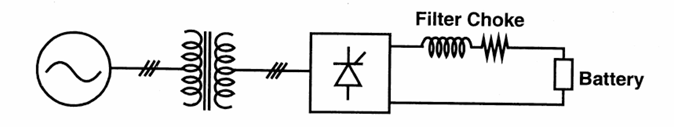
\includegraphics[width=0.7\columnwidth]{figs/Q 54,55.png}\caption{}     \label{fig:myfigure}
\end{figure}
The energy is collected in a bank of 400~V battery and is connected to converter through a large filter choke of resistance 10$\Omega$.

\vspace{1em}

\item \quad The maximum current through the battery will be\hfill{(GATE EE 2011)}

\begin{multicols}{4}
\begin{enumerate}
\item $14 A$
\item $40 A$
\item $80 A$
\item $94 A$
\end{enumerate}
\end{multicols}
\item \quad The kVA rating of the input transformer is\hfill{(GATE EE 2011)}
\begin{multicols}{4}
\begin{enumerate}
\item $53.2 kVA$
\item $46.0 kVA$
\item $22.6 kVA$
\item $19.6 kVA$
\end{enumerate}
\end{multicols}
\vfill
\noindent\rule{\textwidth}{0.4pt}
\raggedright{EE-A}
\hfill
16/24
\newpage
\raggedright{2011}
\hfill
\raggedleft{EE}\\

\noindent\rule{\textwidth}{0.4pt}

\raggedright{\textbf{General Aptitude (GA) Questions}}

\textbf{Q.56 -- Q.60 carry one mark each.}

\item Choose the most appropriate word from the options given below to complete the following sentence: \\
\textbf{Under ethical guidelines recently adopted by the Indian Medical Association, human genes are to be manipulated only to correct diseases for which \rule{2cm}{0.15mm} treatments are unsatisfactory.}\hfill{(GATE EE 2011)}
\begin{multicols}{2}
\begin{enumerate}
\item similar
\item most
\item uncommon
\item available 
\end{enumerate}
\end{multicols}

\item The question below consists of a pair of related words followed by four pairs of words. Select the pair that best expresses the relation in the original pair:\hfill{(GATE EE 2011)} \\
\textbf{Gladiator : Arena}
\begin{multicols}{2}
\begin{enumerate}
\item dancer : stage
\item commuter : train
\item teacher : classroom
\item lawyer : courtroom
\end{enumerate}
\end{multicols}

\item There are two candidates P and Q in an election. During the campaign, 40\% of the voters promised to vote for P, and rest for Q. However, on the day of election 15\% of the voters went back on their promise to vote for P and instead voted for Q. 25\% of the voters went back on their promise to vote for Q and instead voted for P. Suppose, P lost by 2 votes, then what was the total number of voters?\hfill{(GATE EE 2011)}
\begin{multicols}{4}
\begin{enumerate}
\item 100
\item 110
\item 90
\item 95
\end{enumerate}
\end{multicols}

\item Choose the most appropriate word from the options given below to complete the following sentence: \\
\textbf{It was her view that the country's problems had been \rule{2cm}{0.15mm} by foreign technocrats, so that to invite them to come back would be counter-productive.}\hfill{(GATE EE 2011)}


\begin{enumerate}
\item identified
\item ascertained
\item exacerbated
\item analysed
\end{enumerate}

\item Choose the word from the options given below that is most nearly opposite in meaning to the given word:\hfill{(GATE EE 2011)} \\
\textbf{Frequency}
\begin{enumerate}
\item[(A)] periodicity
\item[(B)] rarity
\item[(C)] gradualness
\item[(D)] persistency
\end{enumerate}
\textbf{Q.61 to Q.65 carry two marks each.}
\item The sum of $n$ terms of the series $4+44+444+\ldots$ is\hfill{(GATE EE 2011)}
\begin{multicols}{2}
\begin{enumerate}
\item $\frac{4}{81} \left[10^{n+1} - 9n - 1\right]$ \\
\item $\frac{4}{81} \left[10^{n-1} - 9n - 1\right]$ \\
\item $\frac{4}{81} \left[10^{n+1} - 9n - 10\right]$ \\
\item $\frac{4}{81} \left[10^{n} - 9n - 10\right]$
\end{enumerate}
\end{multicols}

\newpage
\raggedright{2011}
\hfill
\raggedleft{EE}\\
\noindent\rule{\textwidth}{0.4pt}

\item \textbf{The horse has played a little known but very important role in the field of the medicine.Horses were injected with toxins of diseases until their blood built up immunities.Then serum was made from their blood.Serums to fight with diphtheria and tetanus were developed this way.}\\
It can be inferred from the passage, that horses were\hfill{(GATE EE 2011)}

\begin{enumerate}
\item given immunity to diseases
\item generally quite immune to diseases
\item given medicines to fight toxins
\item given diphtheria and tetanus serums
\end{enumerate}
\item The fuel consumed by a motorcycle during a journey while travelling at various speeds is imdicated in the graph below.\hfill{(GATE EE 2011)}
\begin{figure}[H]
    \centering
    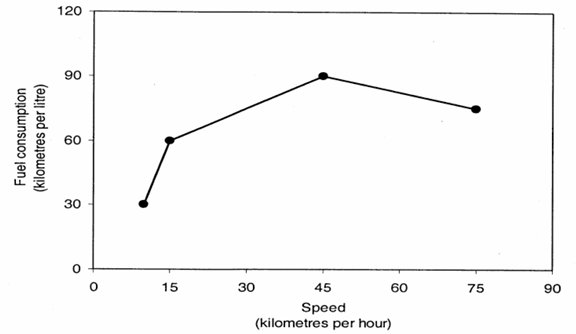
\includegraphics[width=0.6\columnwidth]{figs/Q 63.png}\caption{}     \label{fig:myfigure}
\end{figure}
The distances covered during four laps of the journey are listed in the table below\\

\centering{
\begin{tabular}{|c|c|c|}
\hline
\textbf{Lap} & \begin{tabular}[c]{@{}c@{}}Distance\\ (kilometres)\end{tabular} &
\begin{tabular}[c]{@{}c@{}}Average speed\\ (kilometres per hour)\end{tabular} \\ \hline
P & 15 & 15 \\ \hline
Q & 75 & 45 \\ \hline
R & 40 & 75 \\ \hline
S & 10 & 10 \\ \hline
\end{tabular}}\\
From the given data, we can conclude that the fuel consumed per kilometre was least during the lap
\begin{multicols}{4}
\begin{enumerate}
\item P
\item Q
\item R
\item S
\end{enumerate}
\end{multicols}
\item Three friends, R, S and T shared toffee from a bowl. R took $\frac{1}{3}rd$ of the toffees, but returned four to the bowl. S took $\frac{1}{4}rd$th of what was left but returned three toffees to the bowl. T took half of the remainder but returned two back into the bowl. If the bowl had 17 toffees left, how many toffees were originally there in the bowl?\hfill{(GATE EE 2011)}
\begin{multicols}{4}
\begin{enumerate}
\item 38
\item 31
\item 48
\item 41
\end{enumerate}
\end{multicols}
\item Given that$ f(y)=|y|/ y$, and q is any non-zero real number, the value of $ |f(q) - f(-q) |$
 is\hfill{(GATE EE 2011)}
\begin{multicols}{4}
\begin{enumerate}
\item 0
\item -1
\item 1
\item 2
\end{enumerate}
\end{multicols}

\centering{\textbf{END OF THE QUESTION PAPER}}
\vfill
\noindent\rule{\textwidth}{0.4pt}
\raggedright{EE-A}
\hfill
18/24



\end{enumerate}

\end{document}




    \myvec{
    }